\begin{itemize}
    \item é un elemento che è in grado di indicare L'Elemento successivo in una struttura dati
    \item I Funzioni:
    \begin{itemize}
        \item  \textbf{\textcolor{blue}{\code{Lettura del dato nell’elemento;}}}
        \item  \textbf{\textcolor{blue}{\code{Controllo di terminazione;}}}
        \item  \textbf{\textcolor{blue}{\code{Successore (++);}}}
        \item  \textbf{\textcolor{blue}{\code{Ripristinare la radice}}} (ma solo nei \code{ResettableIterator}) o comunque il punto di inizio
    \end{itemize}
\end{itemize}

\subsection{Iteratori per i alberi}
Abbiamo diversi modi per visitare un albero:
\begin{itemize}
    \item \textbf{Visita in ampiezza}
    \item \textbf{Visita in profondità}
\end{itemize}
\subsubsection{Visita in ampiezza}
\begin{itemize}
    \item Abbiamo bisogno di una \textcolor{blue}{\code{coda}} di supporto per:
    \begin{itemize}
        \item \textbf{\textcolor{blue}{\code{Lettura del dato}}}: metodo della classe;
        \item \textbf{\textcolor{blue}{\code{Controllo di terminazione}}}: controlla se la coda è vuota;
        \item \textbf{\textcolor{blue}{\code{Sucessore}}}: Dequeue del nodo visitato e Enqueue dei due figli del nodo corrente.
    \end{itemize}
    \begin{center}
        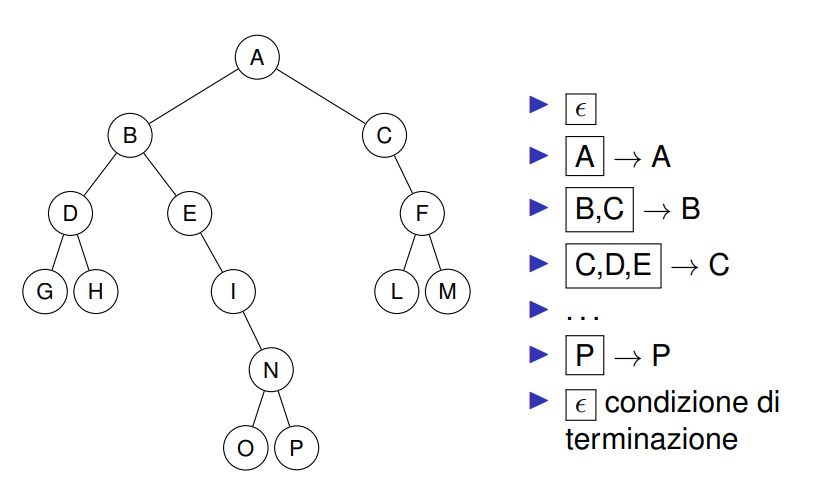
\includegraphics[scale = 0.5]{Capitoli/Iteratori/Esempi/Visita in ampiezza.png}
    \end{center}
\end{itemize}

\subsubsection{Visita in profondità}
Abbiamo tre modi per visitare in profondità:
\begin{itemize}
    \item \textbf{\textcolor{blue}{\code{Preorder}}}
    \item \textbf{\textcolor{blue}{\code{Inorder}}}
    \item \textbf{\textcolor{blue}{\code{Postorder}}}\newline\newline
\end{itemize}
Ci serve uno \textcolor{blue}{\code{Stack}} di supporto per la visita \textbf{\textcolor{blue}{\code{PreOrder}}}:
\begin{itemize}
    \item \textbf{\textcolor{blue}{\code{lettura del dato:}}} metodo della classe;
    \item \textbf{\textcolor{blue}{\code{controllo di terminazione:}}} \code{stack} vuoto;
    \item \textbf{\textcolor{blue}{\code{successore:}}} \code{Pop} del nodo visitato e \code{push} dei due figli del nodo corrente.
    \begin{center}
        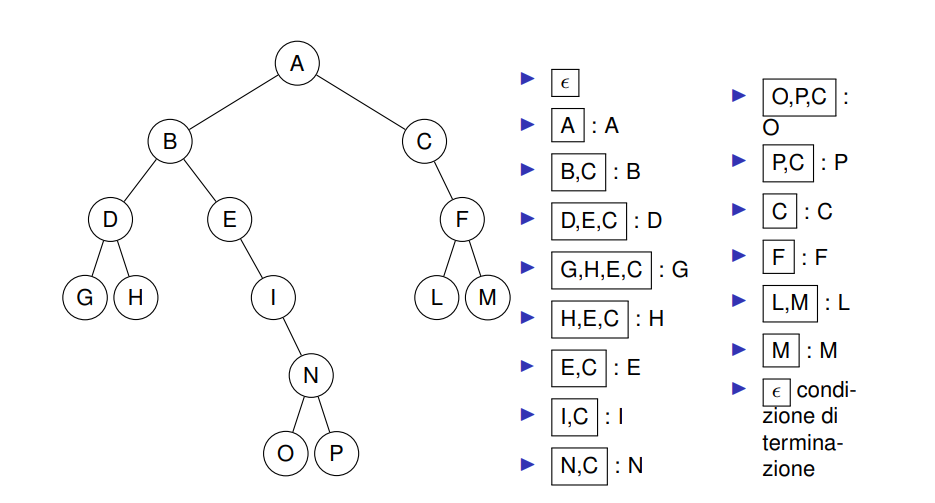
\includegraphics[scale = 0.6]{Capitoli/Iteratori/Esempi/visita PreOrder.png}
    \end{center}
    \begin{tcolorbox}[width=15cm, boxsep=10pt]
        \item \textbf{Codice Visita PreOrder:}
        \lstinputlisting{Capitoli/Iteratori/Esempi/CodicePreOrder.txt} 
    \end{tcolorbox}
\end{itemize}
\newpage
\textbf{Visita} \textbf{\textcolor{blue}{\code{InOrder}}}:
\begin{itemize}
    \item  In questo caso il \textbf{nodo corrente} viene scoperto, ma non
   \textbf{ ancora visitato}: prima bisogna visitare il \textbf{sottoalbero}
    \textbf{sinistro}.
    \item Solito \code{stack} di supporto.
    \item \code{searchLeftMostNode} Ci serve anche una funzione che
    continua a scendere a sinistra fino a quando possibile
    inserendo man mano i nodi che incontra nello stack: si
    ferma al primo nodo il cui figlio sinistro è vuoto.
    \item scopri Quando scopriamo un nodo, ne facciamo il \code{push}
    nello \code{stack} e poi scendiamo a sinistra con
    \code{searchLeftMostNode}
    \begin{itemize}
        \item \textbf{\textcolor{blue}{\code{lettura del dato:}}} metodo della classe;
        \item \textbf{\textcolor{blue}{\code{controllo di terminazione:}}} stack vuoto;
        \item \textbf{\textcolor{blue}{\code{successore:}}} Pop e restituisco il nodo; visita il suo nodo
        destro, se c’è.
    \end{itemize}
    \item Naturalmente parto dalla radice dell’albero.
    \begin{center}
        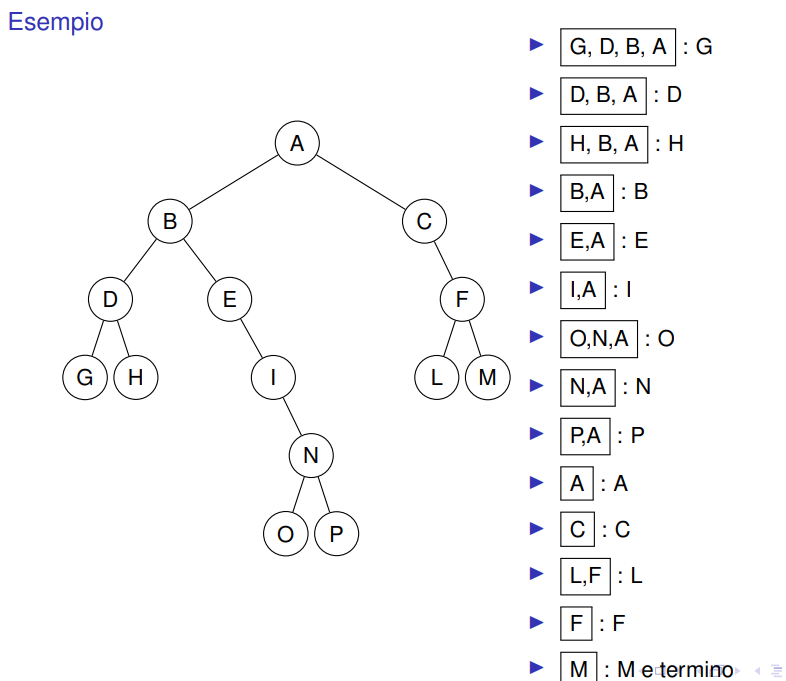
\includegraphics[scale = 0.6]{Capitoli/Iteratori/Esempi/Visita InOrder.png}
    \end{center}
\end{itemize}
\textbf{Visita} \textbf{\textcolor{blue}{\code{PostOrder}}}:
\begin{itemize}
    \item È un poi’ più complicato, perché la strategia cambia a
    seconda che stia risalendo l’albero da destra o da sinistra:
    per capirlo devo tenere l’ultimo nodo restituito, che
    chiameremo \code{current}.
    \item La visita di un nodo implica fare il \code{Pop} del nodo e poi
    scendere a sinistra con \code{searchLeftMostList}: quando
    trova un nodo col figlio sinistro vuoto, salta al destro e
    rincomincia a sinistra, fino a quando non trova una foglia.
    \begin{itemize}
    \item \textbf{\textcolor{blue}{\code{lettura del dato:}}} metodo della classe;
    \item \textbf{\textcolor{blue}{\code{controllo di terminazione:}}} \code{stack} vuoto;
    \item \textbf{\textcolor{blue}{\code{successore:}}} ripeti fino a quando non arrivi ad un \code{Pop} e
    restituisci:
        \begin{itemize}
            \item se \code{current == figlio sinistro} del \code{Top} dello \code{stack}, allora
            scopri il \textbf{figlio destro};
            \item se \code{current == figlio destro} del \code{Top} dello \code{stack}, \code{Pop} e
            \textbf{restituisci}
            \item altrimenti (foglia), \code{Pop} e \textbf{restituisci}
        \end{itemize}
    \end{itemize}
    \item Naturalmente parto dalla radice dell’albero.
    \begin{center}
        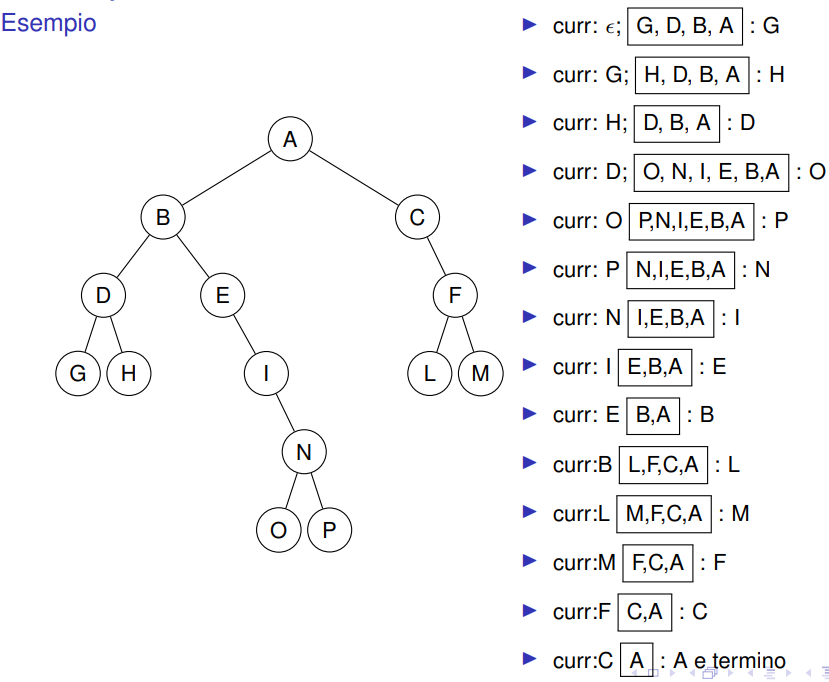
\includegraphics[scale = 0.5]{Capitoli/Iteratori/Esempi/Visita PostOrder.png}
    \end{center}
\end{itemize}